\documentclass[11pt,a4paper,openright,twoside]{report}

\usepackage[pdftex]{graphicx}
\usepackage[english]{babel}
\usepackage[T1]{fontenc}
\usepackage[utf8]{inputenc}
\usepackage{url}
\usepackage[hidelinks]{hyperref}
\usepackage{setspace}
\usepackage{mwe}
\usepackage{pdfpages}
\usepackage{longtable}
\usepackage{tabularx,ragged2e,booktabs,caption}

\usepackage{fancyhdr}
\usepackage{indentfirst}
\usepackage{newlfont}
\usepackage{xcolor}

\definecolor{mygreen}{rgb}{0,0.6,0}
\definecolor{mygray}{rgb}{0.5,0.5,0.5}
\definecolor{mymauve}{rgb}{0.58,0,0.82}
\definecolor{pred}{rgb}{0.9,0,0}
\definecolor{light-gray}{gray}{0.95}
\usepackage{listings}
\lstset{ 
	backgroundcolor=\color{light-gray},   % choose the background color; you must add \usepackage{color} or \usepackage{xcolor}; should come as last argument
	breakatwhitespace=false,         % sets if automatic breaks should only happen at whitespace
	breaklines=true,                 % sets automatic line breaking
	escapeinside={\%*}{*)},          % if you want to add LaTeX within your code
	extendedchars=true,              % lets you use non-ASCII characters; for 8-bits encodings only, does not work with UTF-8
	keepspaces=true,                 % keeps spaces in text, useful for keeping indentation of code (possibly needs columns=flexible)
	basicstyle=\footnotesize,        % the size of the fonts that are used for the code
	numbers=left,                    % where to put the line-numbers; possible values are (none, left, right)
	numbersep=5pt,                   % how far the line-numbers are from the code
	%language=XML,                	 % the language of the code
	commentstyle=\color{mygreen},    % comment style
	keywordstyle=\color{blue},       % keyword style
	numberstyle=\tiny\color{mygray}, % the style that is used for the line-numbers
	%stringstyle=\color{pred},
	rulecolor=\color{black},         % if not set, the frame-color may be changed on line-breaks within not-black text (e.g. comments (green here))
	stringstyle=\color{mymauve},     % string literal style
	tabsize=4		%modify tab space, default too wide
}

\usepackage{amssymb}
\usepackage{amsmath}
\usepackage{latexsym}
\usepackage{amsthm}

\oddsidemargin=30pt \evensidemargin=20pt%impostano i margini
\usepackage[htt]{hyphenat} %per andare a capo nei typescript
\hyphenation{uni-ver-sity
	uni-ver-sit-ies
	how-ever
	ma-nu-script
	ma-nu-scripts
	re-ci-pro-city
	through-out
	some-thing
	al-tern-ate}%serve per la sillabazione: tra parentesi 

\pagestyle{fancy}\addtolength{\headwidth}{20pt}
\renewcommand{\chaptermark}[1]{\markboth{\thechapter.\ #1}{}}
\renewcommand{\sectionmark}[1]{\markright{\thesection \ #1}{}}
\rhead[\fancyplain{}{\bfseries\leftmark}]{\fancyplain{}{\bfseries\thepage}}
\cfoot{}

%\linespread{1.3}                     

\begin{document}
	
	
\includepdf{title-by-itself}
	\clearpage{\pagestyle{empty}\cleardoublepage}%non numera l'ultima pagina sinistra
	
	\tableofcontents                        
	\clearpage{\pagestyle{empty}\cleardoublepage}
	\pagenumbering{arabic}                  %mette i numeri arabi

	\chapter{Introduction}
\label{Intro}
\thispagestyle{empty}

\noindent Bluetooth Low Energy devices are flooding the market of cheap, wearable, health, home-appliance electronics. Some examples include monitoring devices for sport, health and outdoor activities in general; they also connect many household appliances as well as security cameras and locks. Other interesting use-cases include wristbands used in theme parks or live music concerts (although the technology may differ).

Intrinsically, these devices perform very simple tasks, mostly in the field of data gathering. It seems totally harmless to have a smart watch tracking your position at any time of day, but what if it were possible for anyone to query it and extract its data? Their minimalism is what makes them so appealing to the general public, but it is sometimes their intrinsic weakness.

Moving a bit further from \textit{"hackers"} and information security, data gathering is a fundamental step for data analysis in a Big Data context. Privacy concerns should be taken into consideration also in terms of data anonymization.

In this project report, we will start by describing general device characteristics and Bluetooth specifications. We will then move to their concrete observation with hands-on analyses, taking into consideration different developing tools and devices. In particular, we will focus our attention on security risks and concrete flaws, highlighting security exploits when possible. Finally, we will summarize our findings, including a few ideas for future directions and developments.

For our tests, we used a Mi Band 2 smart band, a Magic Blue smart lightbulb and a ST Microelectronics IoT node (model \texttt{B-L475E-IOT1A2 Discovery kit}). The code was run both on Ubuntu 16.04 and Kali Linux 4.13. It is worth mentioning that we also tried to use a Ubuntu GNOME OS, virtualized via VMWare on Windows 10, but this option was soon discarded as VMWare does not provide the drivers for Bluetooth Low Energy. Another requirement is that Bluetooth adapters on the smartphone or laptop must support Bluetooth version 4.0 or higher, as it includes for the first time the LE specification.

The software at our disposal included the builtin Linux commands, as well as Wireshark and Android apps (namely BLEScanner and nRFConnect). As we will see, we also tested some open-source tools available from Github: bleah, btlejuice and gattacker.
	% !TeX spellcheck = en_GB
\chapter{Bluetooth Low Energy Specification}
\label{chapter2}
\thispagestyle{empty}

\noindent In this chapter we briefly report the main technical characteristics of the Bluetooth Low Energy Personal-Area-Network technology. Our main reference is the Core Specification 5.0 available on the official website.

\section{Network Topology and Devices}
Devices can be divided into three categories: Advertisers, Scanners and Initiators. 
Communication has to be started by an initiator device following an \textit{advertisement connectable packet} (\texttt{ADV\_IND}). Advertisement is performed on the primary channels, while bidirectional communication happens on one of the 37 secondary channels, decided during the connection procedure. When a connection is established, the initiator and the advertiser respectively become the master and slave devices; while the former can be involved in more than one communication, the slave device can belong to a single \textit{piconet} at a time. In fact, it is not possible to have a BLE device paired with more than one "master" device at the same time.

Advertising may also be \textit{non-connectable} (\texttt{ADV\_NONCONN\_IND}): the LE device periodically sends its data on the main channel for every scanner to read. This is really convenient in terms of implementation, but it also represent the least secure solution, as data is sent in clear text.

On the whole, the Specification defines six different advertising packets, among which we also report the request for additional information from the advertisement (\texttt{SCAN\_REQ}), it having a direct corresponding bash command.

\section{Decypher Advertising Packets}
Before considering Man-In-The-Middle techniques, we show how it is possible to intercept data from advertising devices, mentioned in the previous chapter.

For this experiment, we used the STM IoT node and tested it on both our Linux distributions. The board simply worked as a thermometer, measuring the temperature in the environment and broadcasting it as a non-connectable advertising packet.
	\chapter{Hacking BLE devices}
\label{chapter3}
\thispagestyle{empty}

\noindent This chapter is dedicated to BLE traffic analysis between two BLE devices. First, we will show how we analysed, reverse-engineered and hacked a Magic Blue smart bulb, with the aid of a mobile phone. It is possible to download the Android application which works as an interface with the BLE device; we also used Wireshark 2.6.2 to easily process captured traffic.This tool is unable to sniff BLE packets unless another support is provided (like Ubertooth or Nordic Semiconductor dongle), so we decided to use Android Developer Tools to register incoming and outgoing Bluetooth traffic.
Through this setting, it becomes easy to track all the packets from the phone to the smart bulb in a single log file. 

In the second example, we developed our own code on the Mbed Online Compiler and tested it on the STM IoT Node. We then tried to connect to the board from different interfaces (as our laptop's or mobile phone's) and used Wireshark to capture and interpret the traffic.

\section{Case study: Smart Bulb}
\subsection{Connect to the device}

The first step in order to sniff packets from a device requires to know its MAC address and understand its profile is structure. There are many open-source tools to accomplish this task, e.g. \texttt{hcitool}, \texttt{bluetoothctl} and \texttt{gatttool}. They come within the Bluez stack and can be easily used from the command line, where Bluez is the official Linux Bluetooth Protocol and provides support for Bluetooth Layers and Protocols. Due to its modularity, it is easy to install the needed modules and libraries, and quickly get to work with devices. In Listings \ref{list:conn-hcitool}, \ref{list:conn-bluetoothctl}, \ref{list:conn-gatttool} we show some possible usages of these three tools.

Among other possibilities, it is worth mentioning a widespread Python implementation called \texttt{bluepy}, which provides an interface for the same functionalities and allows constructing more complex programs.

In conclusion, they all provide similar functions and the user can choose depending on her specific requirements and targets. In this project, the main objective was to scan the surroundings for BLE and BT devices, connecting to them and gathering information about their services and characteristics.

Following are the command lines to scan and connect to the devices.
\lstinputlisting[caption={Connect to device via \texttt{hcitool}.},label={list:conn-hcitool},language=bash]{lescan-connect.txt}
\lstinputlisting[caption={Connect to device via \texttt{bluetoothctl}.},label={list:conn-bluetoothctl},language=bash]{bluetoothctl-connect.txt}
\lstinputlisting[caption={Connect to device via \texttt{gatttool}.},label={list:conn-gatttool},language=bash]{gatttool_connect.txt}

We chose to use \texttt{gatttool} due to its efficiency in displaying the characteristics and services of the target device. Consequently, we will only consider this tool in further project developments and code excerpts.

A connection can be established simply via the \texttt{connect} keyword; afterwards it is possible to explore the characteristics (all of them or only the primary ones) of the device. We have reported the output of the connection process, together with an example of primary services for the smart bulb (see Appendix \ref{appendixB}). However, as the code shows, it is impossible to understand the meaning and purpose of each characteristic, and no support is provided by the Bluetooth GATT Services table.

We tested also an alternative way to connect to the smart bulb, employing an Android app as BLEScanner or nRFConnect. To proceed with this approach, turn the Bluetooth on, and in the main page connectible devices will appear: the user can then easily open another tab and explore the content more deeply.

\begin{figure}
	\centering
	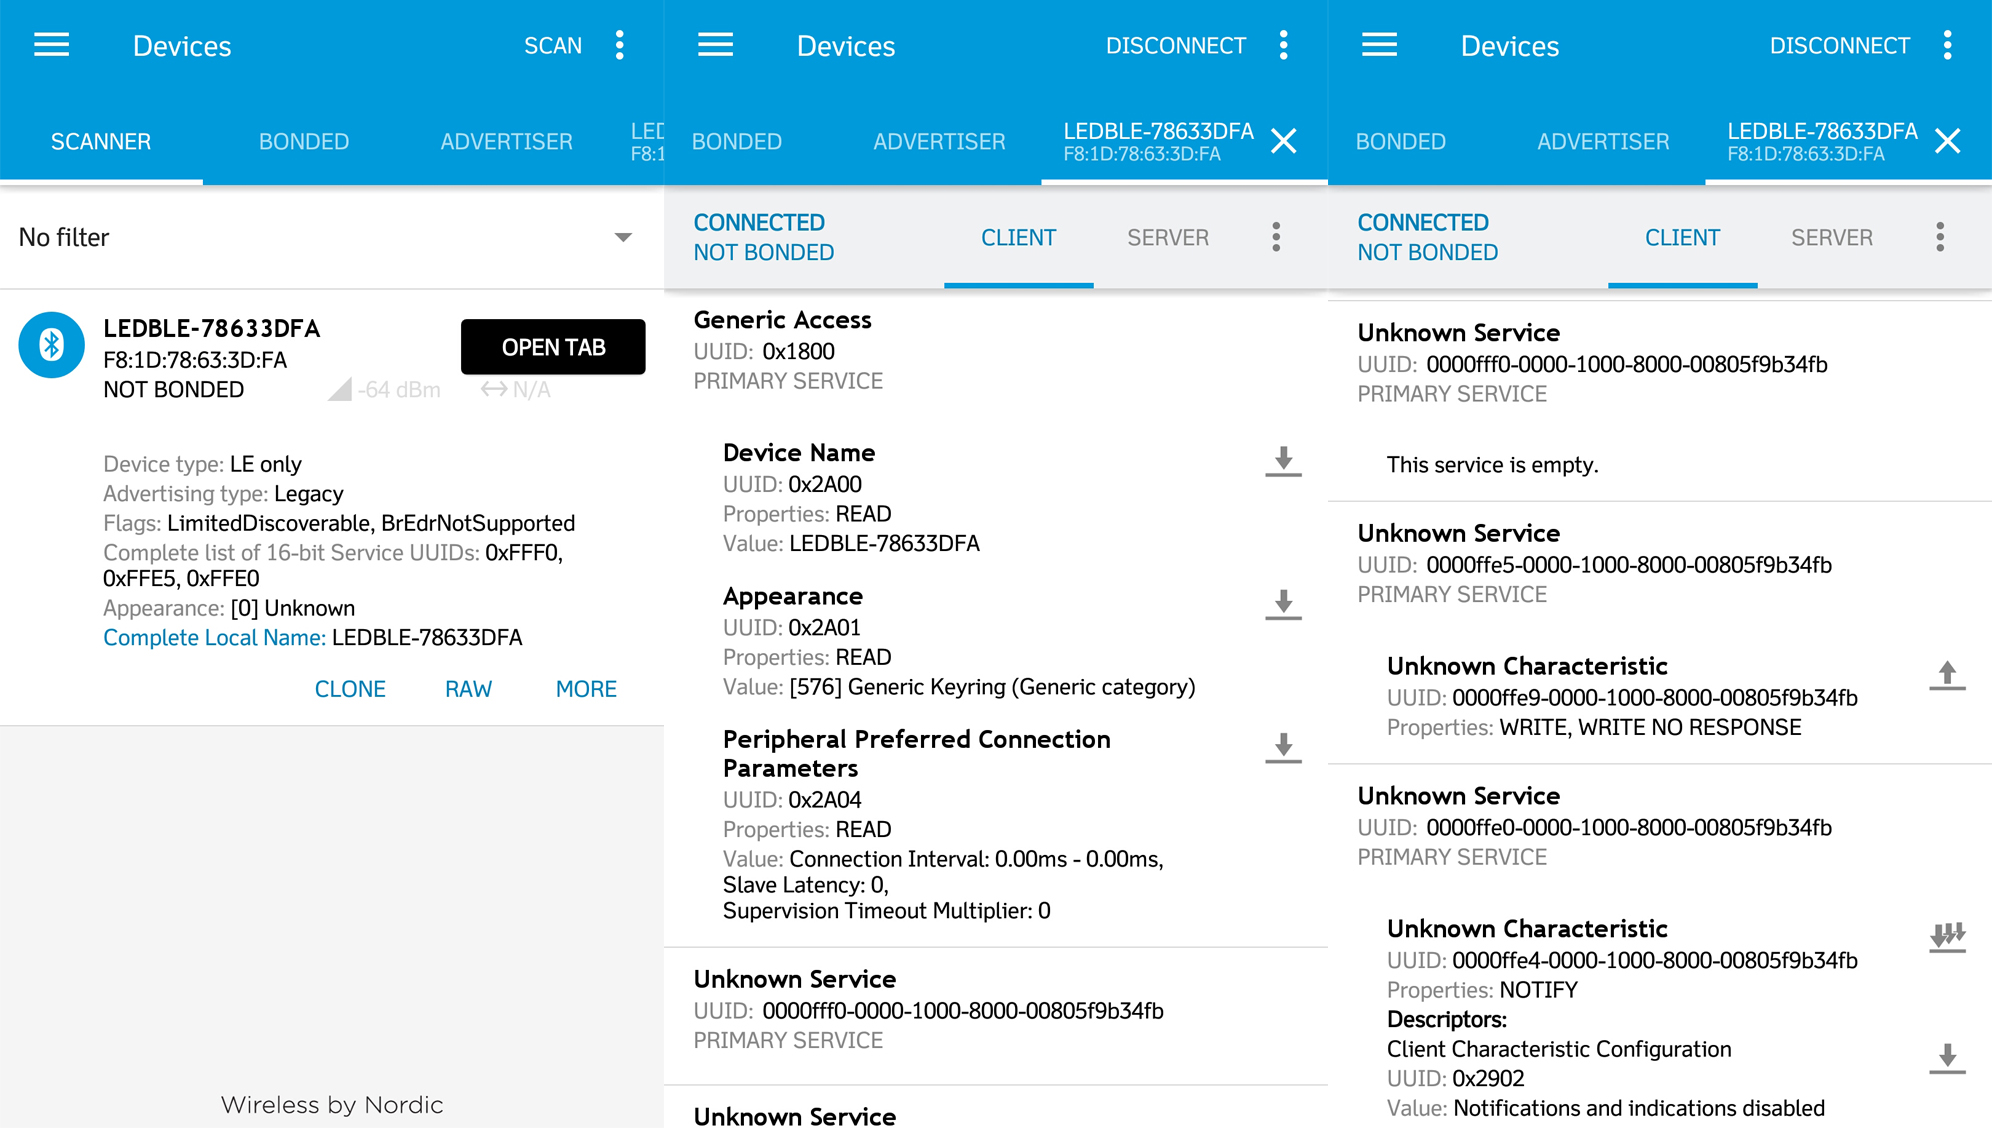
\includegraphics[width=0.9\textwidth]{nrfConnect.jpg}
	\caption{Screenshots from the nRFConnect Android app when connecting to the smart bulb.}
	\label{fig:nrfConnect}
\end{figure}	

Although all the services are labelled as \textit{unknown} and it is not clear what their values mean, the structure of the device profile, including characteristics, services and descriptors is apparent.
It becomes now clear that knowledge of the characteristics and services of a device is not sufficient to understand the meaning of the exchanged data. We thus moved to a different approach: reverse-engineering of the packet structure and content, so to finally understand its meaning. Unfortunately, as previously mentioned, due to the lack of a sniffing device (e.g. a dongle) we decided to use a "legit" way to capture some traffic packets. From Android 4.0 onward, Developer Tools provide the user with a tool to capture all Bluetooth HCI packets in a file, called \texttt{HCI snoop log}. It is important to highlight that this section is not usually available and it has to be activated directly from the user.

In the next step we connect to the MagicBlue app and select the smart bulb from the list of available devices. After pairing, it is possible to choose from a wide range of colours and modes, to modify the brightness and a blinking time interval, as well as to enable the microphone sensitivity or play music from the smart phone and light up the bulb accordingly. Any of these operations requires the phone to send the bulb data packets containing the command requests for the selected function, and all this information is recorded in a snoop log file.
After transferring the file from the phone to a PC, Wireshark is the instrument needed to parse the log file.

\subsection {Traffic Analysis}
One of the obstacles in understanding the structure of data packets exchanged between two BLE devices lies in finding the packets of interest. The amount of data gathered in the log file is indeed impressive, but many of the packets are related to the connection phase between the two entities and so they hold no value for our research.
It is thus advisable to filter on the Bluetooth address of the target device, acquired during the initial scanning phase. Wireshark allows selecting it either via its specific toolbar or via right click, once a meaningful packet has been found. We then proceed to analyse the structure of the remaining packets, leveraging on Wireshark parser, which helps in detecting recurring similarities. We can now understand how the colour information is encoded inside the data structure.

\begin{figure}
	\centering
	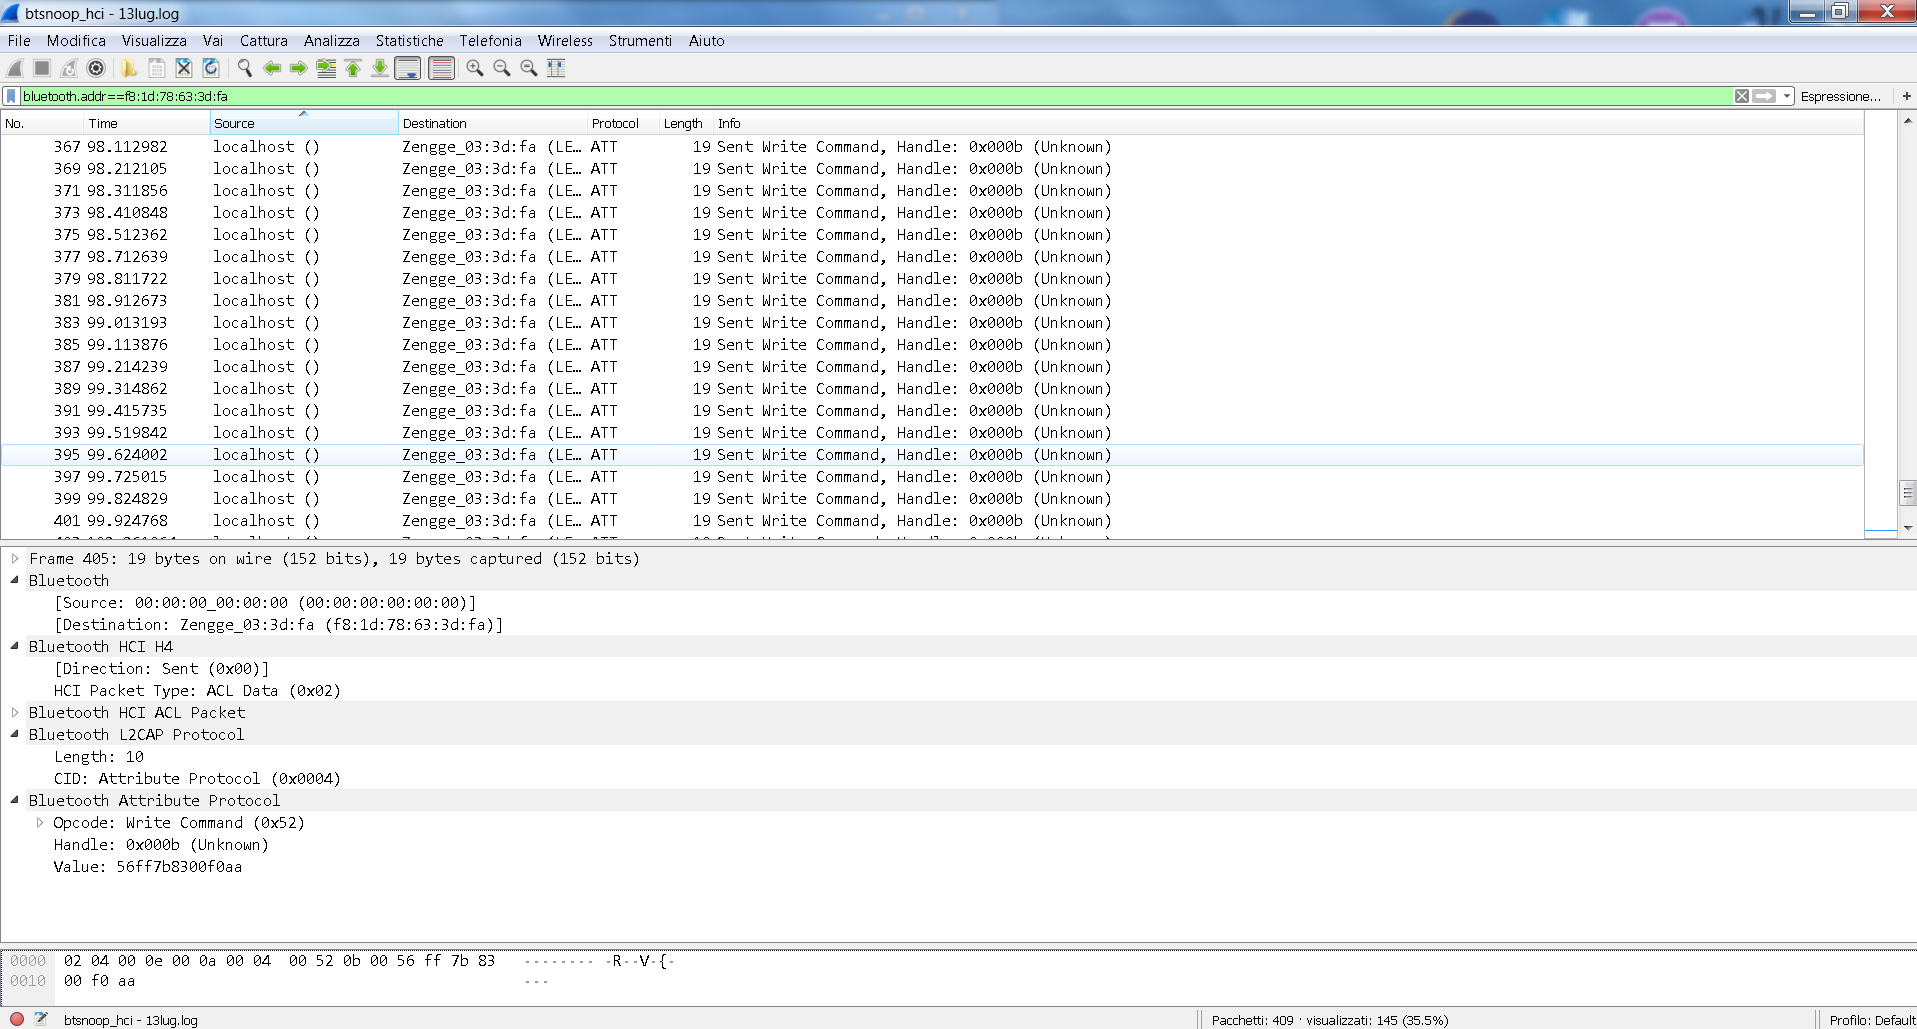
\includegraphics[width=0.9\textwidth]{wireshark1.png}
	\caption{Applying a filter in Wireshark and observing packets contents.}
	\label{fig:wireshark}
\end{figure}

We summarized our findings in the following key considerations.
\begin{itemize}
	\item Within the Attribute Protocol, \texttt{Value} length can be up to a maximum of 20 bytes, depending on the information it transmits.
	\item Writeable Characteristics are usually marked with a ffe9-XX UUID, referring to a ffe5-XX Service.
	\item There are no security layers and it is possible to write any value.
	\item This can be easily accomplished via \texttt{gatttool} or \texttt{bluetoothctl} on the command line, or using a BLE sniffer smart phone app.
\end{itemize}

In tables \ref{tab:colour-blebulb} and \ref{tab:light-blebulb} we provide a short summary of the patterns recognized in Magic Blue smart bulb traffic. The bulb has indeed many more functionalities than the ones reported here, which we did not further investigate.

\begin{minipage}{\linewidth}
	\centering
	\captionof{table}{Single colour choice} \label{tab:colour-blebulb}
	\begin{tabular}{l l} 
		\hline
		Hex value &	Meaning  \\ \hline
		56 &	Fixed prefix  \\ 
		ff085a &	Colour RGB code \\ 
		00 &	From 00 to ff, brightness of the light \\ 
		0f OR f0 &	off/on \\ 
		aa & Fixed suffix  \\ 
		\end {tabular}\par
		\bigskip
\end{minipage}

\begin{minipage}{\linewidth}
	\centering
	\captionof{table}{Light Functions} \label{tab:light-blebulb}
	\begin{tabular}{l l} 
		\hline
		Hex value &	Meaning  \\ \hline
		bb &	Fixed prefix  \\ 
		3 OR 2 &	Respectively active functions \textit{strobo} or \textit{gradual change} \\ 
		0 &	From 00 to ff, brightness of the light \\ 
		1 &	On-time of the lightbulb, from a quick flash (1) to 5 seconds \\ 
		f & Interval of time between flashes (1 faster than f)  \\ 
		44 & Fixed suffix  \\
		\end {tabular}\par
		\bigskip
\end{minipage}

Hacking a smart bulb may be also accomplished by a Python script compiled for a Raspberry Pi device. There is a single requirement on the operating system of the component, as it is needed to install Bluez components as well as a compiler. This solution would allow controlling the device remotely in a continuous way. Moreover, there exists a full Python Compiler called MicroPython for ST Microelectronics, though not compatible with the board used in this project. The list of supported boards is available from the official site.

\section{Case Study: STM IoT Node} 
For this experiment we used the STM IoT node and tested it on both Linux distributions. The board retrieves the temperature and humidity levels in the environment and broadcasts them as a non-connectable advertising packet, as we can see in Listing \ref{list:adv-temp-hum}.
\lstinputlisting[caption={Retrieve sensor values and update packet},label={list:adv-temp-hum},language=c++]{example-temphum.cpp}

Packets broadcasted by the board can be retrieved with any of the tools described at the end of the previous chapter. We analysed the payload and found that it follows this structure:
\begin{center}
	\textit{length - meaning - content}.
\end{center}
The length is expressed in bytes and it refers to the overall size of \textit{meaning} and \textit{content}. The former two is a label which has to be matched with the corresponding Bluetooth GAP Assigned Number (specification available on the website, we report the table in Appendix \ref{appendixA}) to understand its meaning. Common examples are \texttt{0x09} for "Complete Local Name" or \texttt{0x0a} for "Power Level". In our case, the label corresponds to "Service data 16-bit UUID", which means that we should look at the next two bytes to have a more precise indication of the received data. Vendors usually publish a web page in which they list all their codes with the respective meaning, while in this example we can see that its value is added to the payload in \texttt{service\_data[0]}, and corresponds to \texttt{00 aa}.

Finally, the next two bytes encode the temperature and humidity in the room.


	\clearpage{\pagestyle{empty}\cleardoublepage}
	\addcontentsline{toc}{chapter}{Bibliography}
	\bibliographystyle{plainurl}
	\bibliography{bibl_tesi}
	
	\appendix
	
	\pagestyle{fancy} 
	\fancyfoot{}                                               
	\renewcommand{\chaptermark}[1]{\markboth{\appendixname\ \thechapter.\ #1}{}} 
	\renewcommand{\sectionmark}[1]{\markright{\thesection.\ #1}}         
	\fancyhead[LE,RO]{\bfseries\thepage}    
	
	\fancyhead[RE]{\bfseries\leftmark}    
	\fancyhead[LO]{\bfseries\rightmark}     
	\renewcommand{\headrulewidth}{0.3pt} 
	
	\chapter{GATT Assigned Numbers}
\label{appendixA}
\thispagestyle{empty}

\begin{figure}
	\centering
	\begin{minipage}{0.9\textwidth}
		\centering
		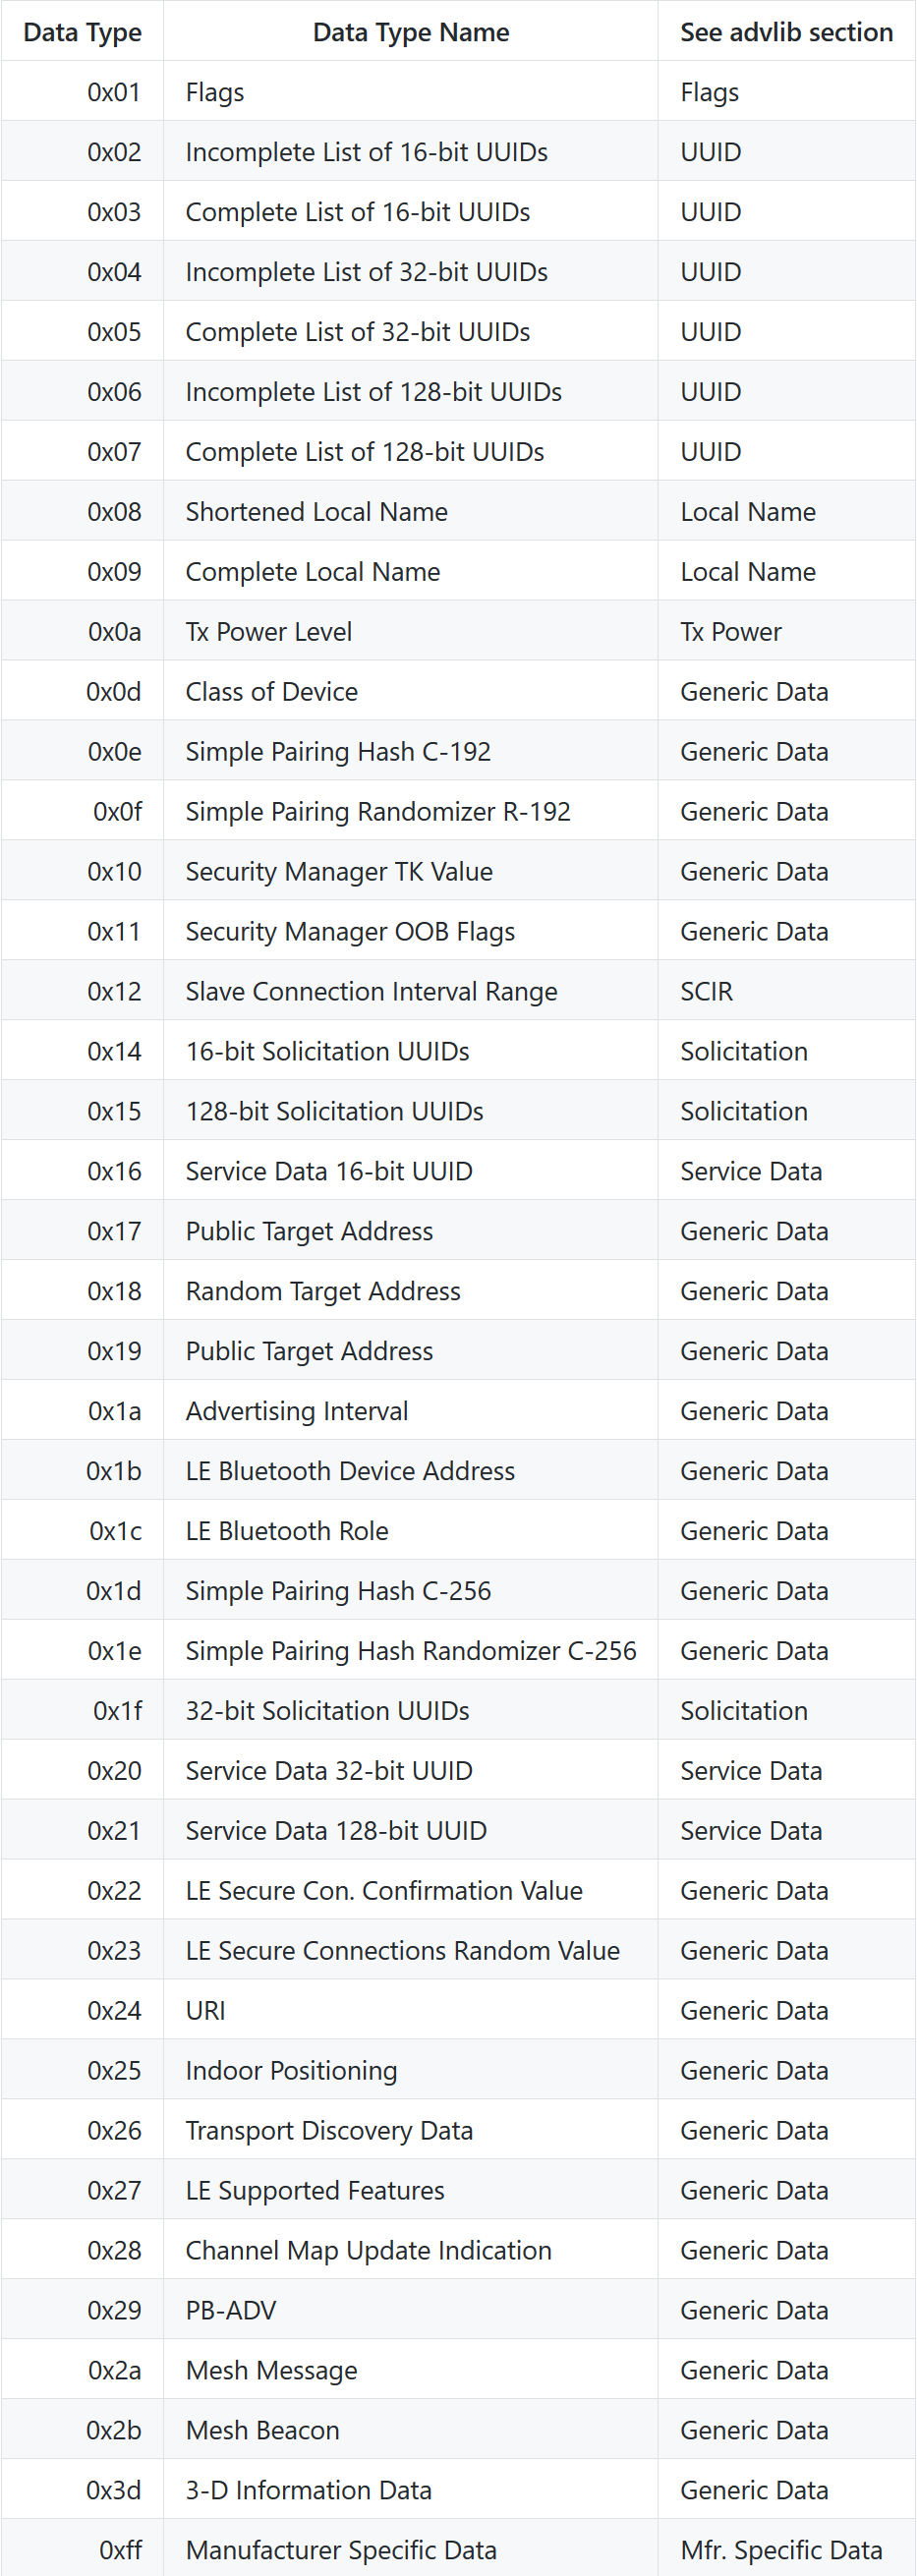
\includegraphics[width=0.8\textwidth]{GAP-assigned-numbers.png}
	\end{minipage}
	\label{fig1-GAP-numbers}
\end{figure}
	\include{AppendixB}

\end{document}
